% Talk of Volume Preserving Mean Curvature Motion
\documentclass[10pt]{beamer}
\usepackage{settings-my-talk}
\includeonlyframes{ slide/frame1,%
                    slide/frame2,%
                    slide/frame3,%
                    slide/frame4,%
                    slide/frame5,%
                   }

%
%
% General Informations
\title{Uno schema Semi-Lagrangiano per il moto per curvatura media che
  preserva il volume}
\author{Michele Cipolla \\
\texttt{cipmiky@gmail.com}}
\institute[Dip. Matematica]{Univeristà la Sapienza di Roma}
\date{23 Luglio 2014}
%\logo{
\includegraphics[width=0.05\textwidth]{logoSapienzaHalf}}
%
%
% Customize Theme
%\definecolor{sapC}{rgb}{0.53,0.15,0.15}
%\usetheme{Antibes}
%\usetheme{Berlin}
%\usetheme{Berkeley}
\usetheme{CambridgeUS}
%\setbeamercolor*{structure}{fg=sapC}
%\setbeamerfont{size=\Large, series=\bfseries,
%  family=\rmfamily}
\setbeamertemplate{headline}
{%
  \begin{beamercolorbox}{section in head/foot}
    \vskip2pt \insertnavigation{\paperwidth}\vskip2pt
   \end{beamercolorbox}
}
\setbeamertemplate{footline}
{%
  \begin{beamercolorbox}{section in head/foot}
    \vskip2pt \insertpagenumber\vskip2pt
   \end{beamercolorbox}
}
%
%
%
\begin{document}
%
%
% Title page
\begin{frame}
\titlepage
\end{frame}
%
%
% Table of contents
\section*{Outline}
\begin{frame}{Outline}
\tableofcontents
\end{frame}
%
%
% Central Frame
\begin{frame}
  \frametitle{Motivazioni}
  \begin{columns}[t]
    \begin{column}{4cm}
       \begin{block}{Deterioramento delle immagini}
         Processi di acquisizione di immagini traminte scanner 3D o di
         trasferimento delle stesse, possono deteriorale generando del
         \alert{rumore}. 
       \end{block}
     \end{column}
     \begin{column}[T]{6cm}
      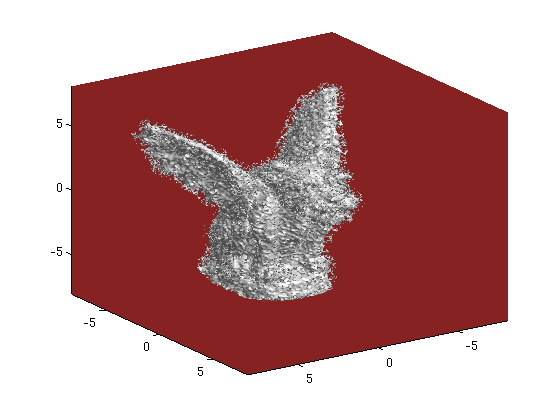
\includegraphics[width=1.0\textwidth]{noise/imnoise/mcm/gargolye/garg149i-0-00}
     \end{column}
  \end{columns}
\end{frame}

\section{Modello}
\begin{frame}{Moto per curvatura media}
     \begin{block}{}
       \begin{itemize}
       \item $S$ superfice regolare in $\mathbb{R}^3$
       \item $\mathcal{S}(p,t)$ parametrizzazione di $S$
       \item $\mathcal{N}(x,t)$ vettore unitario normale regolare
       \item $\mathcal{H}=-\Div(\mathcal{N})\mathcal{N}$ vettore curvatura media
       \end{itemize}
     \end{block}
     \begin{block}{}
       $(x_1,x_2,x_3)\in S_t$ evolve seconde il sitema parabolico
       \[
       \left\{
       \begin{aligned}
         &\mathcal{S}_t(p,t)=-\Div(\mathcal{N})\mathcal{N}\text{ $t>0$} \\
         &\mathcal{S}(0)=S
       \end{aligned}
       \right.
       \]
     \end{block}
\end{frame}

\begin{frame}{Collasso in un punto}
  \begin{columns}[c]
    \begin{column}{6cm}
      \begin{block}{Superfici convesse}
       Superfici convesse  evolvono in un
       punto in un tempo finito.
       \end{block}
      \begin{exampleblock}{Evoluzione della Sfera}
        Una famiglia di sfere $\mathcal{S}(p,t)=S^2(R(t))$ con
        $R(0)=R_0$, si evolve secondo
        \[
        \begin{aligned}
          \overset{\displaystyle.}{R}(t) &= -\frac{2}{R(t)},\,
          R(0)=R_0,\Rightarrow\\
          R(t)&=\sqrt{R_0^2-4t}\Rightarrow, \\
          R(t)&=0 \Longleftrightarrow t=\frac{R_0^2}{4}<\infty 
        \end{aligned}
        \]
      \end{exampleblock}
    \end{column}
    \begin{column}[c]{4cm}
       \begin{center}
     \only<2->{\animategraphics[autoplay,loop,width=1.0\textwidth,height=0.45\textheight]{0.8}{smooth/mcm/sphere/sphere50-}{0}{4}}
     \end{center}
    \end{column}
    \end{columns}
\end{frame}

\begin{frame}{Possibili cambiamenti topologici e singolarità}
  \begin{columns}[c]
    \begin{column}{5cm}
      \begin{block}{Superfici non convesse}
       Superfici non convesse possono subire cambiamenti topologici
       generando delle singolartà. 
       \end{block}
      \begin{exampleblock}{Evoluzione del Manubrio}
        Il manubrio può essere considerato come due sfere di equal
        raggio connesse da un cilindro. A causa del collasso del
        cilindro in una linea, il manubrio si spezza in due sfere
        disconnesse.
      \end{exampleblock}
    \end{column}
    \begin{column}[c]{5cm}
       \begin{center}
     \only<2->{\animategraphics[autoplay,loop,width=1.0\textwidth,height=0.45\textheight]{0.8}{smooth/mcm/dumbbell/dumbb100-}{0}{5}}
     \end{center}
    \end{column}
    \end{columns}
\end{frame}


\begin{frame}{Flusso \emph{volume preserving}}
  \begin{columns}[T]
    \begin{column}{6cm}
      \begin{block}{Processo di nomalizzazione}
        Cambiamo la scala temporale
        \begin{itemize}
        \item $\mathcal{\tilde{S}(\tau)}=\psi(t)\mathcal{S}(t)$ 
        \item $\psi^2(t)=\frac{\partial\tau}{\partial t}$
        \end{itemize}
         in modo tale che \alert{$Volume_{\tau}\equiv 0$}, ottenendo   
         \begin{itemize}
         \item $\mathcal{\tilde{S}}_t=\left(\mathcal{\tilde{H}}-\frac{\rho\iint\mathcal{\tilde{H}}d\mu}{3V_0}\right)\mathcal{N}$
         \item $\rho =-<\mathcal{\tilde{S}},\mathcal{N}>$
         \end{itemize}
      \end{block}
    \end{column}
    \begin{column}[T]{4cm}
      \begin{exampleblock}{Evoluzione della sfera}
        \begin{itemize}
        \item $\tau(t)=\int_0^t\frac{T}{T-\tilde{t}}d\tilde{t}$ con
          $T=\frac{R_0^2}{4}$ tempo di 
          collasso
        \item $\tilde{V}=\psi^3(t)V$
        \item $\tilde{V}=\left(\frac{T}{T-t}\right)^{\frac{3}{2}}V$
        \item $V=\frac{4}{3}\pi(R_0^2-4t)^{\frac{3}{2}}$
        \item $\tilde{V}=\frac{4}{3}\pi R_0^3=V_0$
        \end{itemize}
      \end{exampleblock}
    \end{column}
  \end{columns}
\end{frame}

\section{Formulazione level-set}
\begin{frame}{MCM \emph{volume preserving} in forma level-set}
  \begin{block}{Superfici come insiemi di livello}
    La superfice regolare $S$ è rappresentata come il livello $0$ di
    una funzione ausiliaria $u(x)\in C^{\infty}(\Omega)$
    \begin{itemize}
      \item $S=\{x\in\Omega | u(x)=0\}$ e $Du(x)\neq 0$ in $S$
      \item $\mathcal{N}=-\frac{Du(x)}{|Du(x)|}$ vettore normale
        regolare
    \end{itemize}
  \end{block}
  \begin{block}{Equazione in forma level-set}
    La famiglia di curve regolare $S_t$
    \begin{itemize}
      \item $S_t=\{x\in\Omega | u(x,t)=0\}$ con $u(x,t)$ definita in
        $\Omega\times I$ e tale che $Du(x,t)\neq 0$ in $S_t$
      \item $x_0\in S_{t_0}$, $x(t)\in S_t$ curva regolare in
        $I_{\delta}(t_0)$ tale che $x(t_0)=x_0$
      \item $u(x(t),t)=0$ derivando \alert{velocità normale}$=\frac{u_t(x_0,t_0)}{|Du(x_0,t_0)|}$
    \end{itemize}
  \end{block}
\end{frame}

\begin{frame}{Flusso VPMCM}
  In forma level-set abbiamo
    \[
      (\text{VPMCM})\,u_t=|Du(x,t)|\Div\left(\frac{Du(x,t)}{|Du(x,t)|}\right)-\frac{\iint\Div\left(\frac{Du(x,t)}{|Du(x,t)|}\right)d\mu}{3V_0}x^tDu(x,t). 
      \]
  \begin{block}{Parte MCM e termine di traporto} 
    \begin{itemize}
    \item parte MCM 
      \[
      |Du(x,t)|\Div\left(\frac{Du(x,t)}{|Du(x,t)|}\right)=tr(P(Du)D^2u)
      \]
      \item $P(Du)=I-\frac{b\otimes }{|b|^2}\,b\in\mathbb{R}^3$
        matrice di proezione sul piano ortogonale a $b$
      \item parte di trasporto, non locale. 
        \[
        \mathcal{I}(\mathcal{H}(u),t)=\frac{\iint\Div\left(\frac{Du(x,t)}{|Du(x,t)|}\right)d\mu}{3V_0}
        \]
     \end{itemize}
  \end{block}
\end{frame}

\begin{frame}{Vantaggi forma level-set}
 \begin{block}{Vantaggi}
   \begin{itemize}
     \item Forma level-set scritta in un sistema di coodinate fisso
     \item I cambiamenti topologici non sono un problema. Topologia di
       $u$ è fissa.
     \item L'emergere di discontinuità, per alcune velocità è ben
       posto nella teoria viscosa
   \end{itemize}
 \end{block}

\end{frame}



\begin{frame}{Problema ben posto nella teoria viscosa}
     \begin{block}{Classe dell'equazione}
       La nostra equazione VPMCM \alert{$u_t+F(x,u,Du,D^2u)=0$}
       rappresenta un PDE parabolico non lineare singolare nei punti in cui
       il grandiente di $u$ si annulla ed è ben posto nella teoria
       delle solulzioni viscose. $F$ del tipo
       \begin{itemize}
         \item $F:\Omega\times\mathbb{R}\times\mathbb{R}^n\times
           S(n)\to\mathbb{R}$, $S(n)$ matrici simmetriche e
           $\Omega\subset\mathbb{R}^n$
         \item $u_t+F(x,r,p,X)=0$
       \end{itemize}
     \end{block}
\end{frame}

\begin{frame}{Soluzioni di viscosità}
  \begin{definizione}
    Sia $\Omega$ aperto di $\mathbb{R}^n$ e $T>0$. Sia $F$ continua in
    $W=\overline{\Omega}\times
    [0,T]\times\mathbb{R}\times\mathbb{R}^n\times S(n)$ a valori in
    $\mathbb{R}$. Sia $\mathcal{O}$ aperto in $\Omega\times(0,T)$.
    \begin{itemize}
      \item Una funzione $u:\mathcal{O}\to\mathbb{R}$ semicontinua
        superiormente è una \alert{sotto
          soluzione viscosa} di 
        \[
        u_t+F(x,t,u,Du,D^2u)=0
        \]
        in $\mathcal{O}$ se per ogni $\phi\in C^2(\mathcal{O})$ e
        $\hat{z}=(\hat{x},\hat{t})\in\mathcal{O}$ tale che $(u-\phi)$ ha
        massimo in $\hat{z}$ allora
        \[
        \phi_t(\hat{z})+F(\hat{z},\phi(\hat{z}),D\phi(\hat{z}),D^2\phi(\hat{z}))\leq 0
        \]
        \item $u$ semicontinua inferiomente e una \alert{sopra
          soluzione viscosa}  in $\mathcal{O}$ se per ogni coppia
          $\phi$ e $\hat{z}$ tale che $(u-\phi)$ ha min in $\hat{z}$
          vale che
          \[
          \phi_t(\hat{z})+F(\hat{z},\phi(\hat{z}),D\phi(\hat{z}),D^2\phi(\hat{z}))\geq 0
          \]
        \end{itemize}
  \end{definizione}
\end{frame}

\begin{frame}{Proprietà di confronto}
  \begin{osservazione}
    Nel caso $F$ non sia continua, la definizione di solulzione
    viscosa continua a valere per l'inviluppo semicontinuo di
    $F$. Ricordiamo che data $h$ definita in $L\subset\mathbb{R}^n$
    \begin{itemize}
    \item  invluppo semicontinuo inferiore $h_*(x)=\lim_{r\to
      0}\inf\{h(y); y\in B_r(x)\cap L\}$ con $x\in\overline{L}$
    \item inviluppo semicontinuo superiore $h^*(x)=\lim_{r\to
      0}\sup\{h(y);y\in B_r(x)\cap L\}$ con $x\in\overline{L}$
    \end{itemize}
  \end{osservazione}
  \begin{block}{Propietà di confronto}
    Se $u$ è una sotto soluzione in $Q=\Omega\times[0,T)$ e
      $v$ una sopra  soluzione sempre in $Q$,  allora $u\leq
      v$ in $\mathcal{O}$ se $u\leq v$ sulla frontiera prabolica 
    \[
    \partial_pQ=\Omega\times\{0\}\cup\partial\Omega\times[0,T).
    \]
  \end{block}
\end{frame}

\begin{frame}{Esistenza e confronto in MCM e VPMCM}
  \begin{block}{Problema risolto}
    Nel caso MCM il flusso $F(p,X)=-tr(P(p)X)$ verifica
    \begin{enumerate}
    \item \alert{propria}: $F(x,r,p,X)\leq F(x,s,p,X)$ per $r\leq
      s$ e $\forall\,p\in\mathbb{R}^n$,$X\in S(n)$
    \item \alert{ellittica degenere}: $F(x,r,p,X)\leq
      F(x,r,p,Y)$ per $X\geq Y$
    \item \alert{geometrica}: $F(x,\lambda p,\lambda X+\sigma
      p\otimes p)=\lambda F(x,p,X)$, $\lambda >0,\sigma\in\mathbb{R}$
    %  \item $-\infty<F_*(x,0,O)=F^*(x,0,O)<\infty$
    \end{enumerate}
    sotto queste propietà valgono risultati di esistenza e confronto.
  \end{block}
  \begin{block}{Non abbiamo risultati definitivi}
    Nel caso VPMCM $F(x,u,p,X)=-tr(P(p)X)+b(u)x^tp$. In generale
    $b(u)$ non è costante quindi per esempio non è
    \alert{propria} è neanche \alert{giometrica}, sopravvive solo la
    proprietà di \alert{degenere ellitticità}; per cui  non possiamo
    utilizzare i risultati precedenti. Risultati definitivi su
    questi tipi di equaizioni ancora non ci sono.
  \end{block}
\end{frame}

\section{Schema Numerico Semi-Lagrangiano}
\begin{frame}{Strumenti iniziali}
  \begin{itemize}
    \item $\Omega$ dominio limitato in $\mathbb{R}^3$
    \item $S$ superficie regolare chiusa in forma level-set
    \item $S=\{x\in\Omega; u(x)=0\}$ rappresenta l'\alert{interfaccia} al
      livello zero. 
    \item $\Omega^{-}=\{x\in\Omega; u(x)<0\}$
    \item $\Omega_{+}=\{x\in\Omega; u(x)>0\}$
  \end{itemize}

  \begin{center}
  \tdplotsetmaincoords{60}{40}
  \begin{tikzpicture}[tdplot_main_coords,gray,thick]
    \definecolor{sapC}{rgb}{0.54,0.14,0.14}
    \coordinate (O) at (0.66,0.0,0.0);
       
    \tdplotsetcoord{P}{1.3}{90}{45};
    \tdplotsetcoord{P2}{-2.0}{120}{30};
    \tdplotsetcoord{P3}{3.0}{60}{40};
    \tdplotsetcoord{P4}{0.8}{97}{153};
    \tdplotsetcoord{P5}{1.3}{-55}{40};

    
    \draw [->,sapC](P2) to[out=120,in=180](P5);
    \node[fill=red!15,rotate=50,scale=4.0,rounded corners] at (P4) {};
    \node[shape=circle,draw=gray,fill=gray,inner sep=0pt,minimum size=1mm]
    (origin) at (O) {};
    \node [left,sapC] at (origin.south) {$O$};
    \node[] (end) at (P3) {};
    \node [sapC] at (end.south) {$\Omega^+$};
    \node[] (end1) at (P) {};
    \node [sapC] at (end1.south) {$\Omega^-$};
    \node[] (end2) at (P2) {};
    \node [sapC] at (end2.north) {$S$};

    \draw  [tdplot_main_coords,dashed] (O) ellipse (42pt and 20pt);
    \tdplotsetthetaplanecoords{40};
    \draw [thick,tdplot_rotated_coords](1.0,0.5,0.5) arc (0:360:1.5);
    
        
  \end{tikzpicture}
 \end{center}
\end{frame}

\begin{frame}{Riscriviamo l'integrale nel termine del trasporto}
     L'integrale
    $\iint_{S}\Div\left(\frac{Du}{|Du|}\right)d\mu$ lo
    possiamo riscrivere come per $Du\neq 0$
    \[
    \int_{\Omega}\Div\left(\frac{Du}{|Du|}\right)|Du|\delta(u)dx
    \]
    \begin{itemize}
    \item L'integrale di superficie di una funzione $f(x)$ si può
      definire anche come 
      \[
      \int_{\Omega}f(x)\hat{\delta}(x)dx
      \]   
    \item $\hat{\delta}(x)=DH(u(x))\cdot\mathcal{V}$ delta
      multidimensionale con $\mathcal{V}$ normale esterna ed 
      \[
      H(u(x))=
      \begin{cases}
        0 &\text{ se }u\leq 0 \\
        1 &\text{ se }u > 0
      \end{cases}
      \]
    \item $\hat{\delta}(x)=H'(u(x))Du\cdot\frac{Du}{|Du|}=\delta(u)|Du|$
    \end{itemize}
 \end{frame}

\begin{frame}{Riscriviamo il termine MCM}
  Ricordiamo il flusso MCM essere $tr(P(Du)D^2u)$ con
  $P(Du)=I-\frac{Du\otimes Du}{|Du|^2}$
  \begin{enumerate}
    \item $P(Du)$ matrice di proiezione sul piano tangente alla
      superficie, di rango $2$ con due autovettori relativi
      all'autovalore $\lambda=1$ 
    \item  $v_1$ e $v_2$ autovettori ortonormali di $P$ 
      \[
      v_1=
      \begin{bmatrix}
        \frac{-u_{x_3}}{\sqrt{u_{x_1}^2+u_{x_3}^2}} \\
        0 \\
        \frac{u_{x_1}}{\sqrt{u_{x_1}^2+u_{x_3}^2}}
      \end{bmatrix}
      \quad
      v_2=\frac{1}{|Du|}
      \begin{bmatrix}
        \frac{-u_{x_1}u_{x_2}}{\sqrt{u_{x_1}^2+u_{x_3}^2}} \\
        \sqrt{u_{x_1}^2+u_{x_3}^2} \\
        \frac{-u_{x_2}u_{x_3}}{\sqrt{u_{x_1}^2+u_{x_3}^2}}
      \end{bmatrix}
      \]
    \item per $v_1$ e $v_2$ si verifica che 
    \[
    P(Du)=\sum_{i=1}^2v_i\otimes v_i=\sigma\sigma^t\quad\text{con }
    \sigma=[v_1,v_2]\in\mathbb{R}^{3\times 2} 
    \]
  \end{enumerate}
\end{frame}

\begin{frame}{Riscriviamo il flusso MCM}
  \begin{alertblock}{Flusso MCM}
    Vale la seguente uguaglianza
    \[
    F_{\text{MCM}}(Du,D^2u)=v_1^tD^2uv_1+v_2^tD^2uv_2
    \]
  \end{alertblock}
  \begin{block}{Esplicitazione del conto}
  Sostituiamo l'espressione  $P(Du)=\sum_{i=1}^2v_i\otimes
  v_i=\sum_{i=1}^2v_iv_i^t$ nel flusso MCM, ottenendo
  \[
  \begin{aligned}
    tr(P(Du)D^2u)&=tr((v_1v_1^t+v_2v_2^t)D^2u)=\\
    &tr((v_1v_1^t)D^2u+(v_2v_2^t)D^2u).
  \end{aligned}
  \]
  Traccia operatore lineare
  \[
  \begin{aligned}
    F_{\text{MCM}}(Du,D^2u)&=tr((v_1v_1^t)D^2u)+tr(v_2v_2^t)D^2u)=\\
    &v_1^tD^2uv_1+v_2^tD^2uv_2.
  \end{aligned}
    \]
  \end{block}
\end{frame}

\begin{frame}{Schema Semi-Lagrangiano VPMCM}
  \begin{block}{Griglia spaziale e temporale}
    \begin{itemize}
      \item $x_j=(j_1\Delta x,j_2\Delta x,j_3\Delta x)$,
        $j\in\mathbb{Z}^3$ e $t^n=n\Delta t$, $n\in\mathbb{N}$
      \item $(x_j,t^n)$ punto della griglia $G_{\Delta x}\times
        G^{\Delta t}$
      \item $u_j^n$ approssimazione di $u(x_j,t^n)$
      \item $D_j^n$ approssimazione di $Du(x_j,t^n)$
    \end{itemize}
    \end{block}
  \begin{osservazione}
    I vettori $v_1$ e $v_2$ non sono definiti quando $|Du|=0$ o
    $u_{x_1}^2+u_{x_3}^2=0$. Numericamente introduciamo una soglia:
    \begin{itemize}
    \item \alert{sopra la soglia}
      \[
      |D_j^n|>C\Delta x \land (D_j^n)_1^2+(D_j^n)_3^2>C\Delta x
      \]
    \item \alert{sotto la soglia}
      \[
      |D_j^n|\leq C\Delta x \lor (D_j^n)_1^2+(D_j^n)_3^2\leq C\Delta x
      \]
      \end{itemize}
    \end{osservazione}
\end{frame}

\begin{frame}{Schema Semi-Lagrangiano VPMCM}
  \begin{block}{Equazione di partenza}
    \[
    u_t=v_1^tD^2uv_1+v_2^tD^2uv_2 - \frac{\int_{\Omega}F_{\text{MCM}}(Du,D^2u)\delta(u)dx}{3V_0}x^tDu
    \]
  \end{block}
  \begin{block}{Punti principali della costruzione}
    \begin{enumerate}
    \item Approssimazione flusso VPMCM sopra la soglia
    \item Schema \emph{ad hoc} nel caso sotto la soglia
    \item Approssimazione del coefficiente del trasporto $\mathcal{I}$
      al tempo $t$ 
    \end{enumerate}
  \end{block}
\end{frame}
 
\begin{frame}{Approssimazione flusso VPMCM. Caso sopra la soglia}
  \only<1>{\begin{alertblock}{Flusso VPMCM}
    $F_{\text{VPMCM}}=v_1^tD^2uv_1+v_2^tD^2uv_2 -
    \mathcal{I}(u,t)x^tDu$
    \end{alertblock}
  \begin{itemize}
    \item $\mathcal{I}^n$ opportuna approssimazione del coefficiente
      del trasporto al  tempo $t^n$
    \item Differenze finite centrate di passo $\Delta x$ 
      \[
      Du\simeq D_j^n\quad v_1(D_j^n)=v_{j,1}^n\quad v_2(D_j^n)=v_{j,2}^n
      \]
    \item \alert{Flusso MCM}: discretizziamo usando incrementi direzionali
      nelle \alert{quattro} direzioni $(\pm v_1\pm v_2)$ con passo
      $\sqrt{2\Delta t}=\rho$
      \[
      \begin{aligned}
        &F_{\text{MCM}}(Du,D^2u)\simeq\frac{1}{2\rho^2}(u(x_j+\rho(v_1+v_2),t)+u(x_j+\rho(v_1-v_2),t)+\\ 
        &u(x_j+\rho(-v_1+v_2),t)+u(x_j+\rho(-v_1-v_2))-4u_j^n).
      \end{aligned}
      \]
  \end{itemize}}
      \only<2>{
        Serie di Taylor nella direzione $v_1+v_2$ 
          \[
          \begin{aligned}
            &u(x+\sqrt{2\Delta t}(v_1+v_2),t^n)=u(x,t^n)+\\
            &<Du(x,t^n),(v_1+v_2)>\sqrt{2\Delta t}+\Delta
            t<D^2u(x_j,t^n)(v_1+v_2),(v_1+v_2)>+\\
            &+T_3\Delta^{\frac{3}{2}} +O(\Delta t^2)
          \end{aligned}
          \]
          Sviluppando nelle altre direzioni e sommando riusciamo ad
          approssimare il flusso con un errore dell'ordine
          $O(\Delta t^2)$.
          \[
          v_1^tD^2uv_1+v_2^tD^2uv_2 =\frac{1}{4\Delta t}(\sum_{+,-}
          u(x_j+\sqrt{2\Delta t}(\pm v_1 \pm
          v_2),t^n)-4u(x,t))+O(\Delta t^2)
          \]
      }

       \only<3>{ 
         \begin{itemize}
           \item Incrementi nelle \alert{quattro} direzioni $(\pm
         v_1\pm v_2)$ più ci andiamo a ricostruire la parte di
         trasporto indietro lungo la caratteristica
         \[
         %\begin{aligned}
           F_{\text{VPMCM}}\simeq(u(x_j-\Delta t\mathcal{I}^nx_j,t)\dots%+ \\
           %&u(x_j-\Delta t\mathcal{I}^nx_j,t)+\\
           %&u(x_j-\Delta t\mathcal{I}^nx_j,t)+\\
           %&u(x_j-\Delta t\mathcal{I}^nx_j,t))
         %\end{aligned}
         \]
       \end{itemize}}
       \only<4>{
         \begin{itemize}
           \item Incrementi nelle \alert{quattro} direzioni $(\pm
         v_1\pm v_2)$ più ci andiamo a ricostruire la parte di
         trasporto indietro lungo la caratteristica
           \[
         \begin{aligned}
           &F_{\text{VPMCM}}\simeq\frac{1}{4\Delta
          t}(u(x_j-\Delta t\mathcal{I}^nx_j+\sqrt{2\Delta
             t}(v_{j,1}^n+v_{j,2}^n),t)+ \\
           &u(x_j-\Delta t\mathcal{I}^nx_j+\sqrt{2\Delta
             t}(v_{j,1}^n-v_{j,2}^n),t)+\\
           &u(x_j-\Delta t\mathcal{I}^nx_j+\sqrt{2\Delta
             t}(-v_{j,1}^n+v_{j,2}^n),t)+\\
           &u(x_j-\Delta t\mathcal{I}^nx_j+\sqrt{2\Delta
             t}(-v_{j,1}^n-v_{j,2}^n),t)-4u_j^n)
         \end{aligned}
         \]
       \end{itemize}}
\end{frame}

\begin{frame}{Schema SL VPMCM sopra la soglia}
  \begin{alertblock}{VPMCM \emph{fully discrete}}
    \begin{itemize}
    \item Approssimazione coefficiente del trasporto $\mathcal{I}^n$
    \item Differenze finite centrate per $D_j^n$ più
      $v_i(D_j^n)=v_{j,i}^n$
    \item Approssimazione del flusso $F_{VPMCM}$
    \item Differenze finite in avanti per
      $u_t\simeq\frac{u(x_j,t^{n+1})-u(x_j,t^n)}{\Delta t}$
    \item Interpolazione lineare $I[\cdot]$ nei punti
      $x_j(1-\mathcal{I}^n\Delta t)+\sqrt{2\Delta t}(\pm
      v_{j,1}^n\pm v_{j,2}^n)$
    \end{itemize}
    \[
    \begin{aligned}
        u_j^{n+1}&=\frac{1}{4}(I[u^n](x_j(1-\mathcal{I}^n\Delta t)+\sqrt{2\Delta
          t}(v_{j,1}^n+v_{j,2}^n))+ \\
        &I[u^n](x_j(1-\mathcal{I}^n\Delta t)+\sqrt{2\Delta
          t}(v_{j,1}^n-v_{j,2}^n))+\\
        &I[u^n](x_j(1-\mathcal{I}^n\Delta t)+\sqrt{2\Delta
          t}(-v_{j,1}^n+v_{j,2}^n))+\\
        &I[u^n](x_j(1-\mathcal{I}^n\Delta t)+\sqrt{2\Delta
          t}(-v_{j,1}^n-v_{j,2}^n))
    \end{aligned}
    \]
  \end{alertblock}
\end{frame}
 
\begin{frame}{Approssimazione flusso VPMCM. Caso sotto la soglia}
  Nel caso sotto la soglia $|D_j^n|\leq C\Delta x$ o
  $(D_j^n)_1^2+(D_j^n)_3^2\leq C\Delta x$, 
  \[
  u_j^{n+1}=\frac{1}{6}\sum_{i\in D(j)}u_i^n
  \]
con $D(j)=\{j\pm e_i\Delta x\,,i=1,2,3\}$, che rappresenta
l'approssimazione dell'equazione del calore
\[
u_t=\varepsilon \Delta u,\quad \varepsilon=\frac{\Delta x^2}{6\Delta t}
\]
Questo metodo è lo stesso utilizzato nello schema classico MCM e 
risulta consistente con $\underline{F}(Du,D^2u)$ e
$\overline{F}(Du,D^2u)$ suggerite da \emph{Crandall and Lions}.
\[
\underline{F}=
\begin{cases}
-\Div\left(\frac{Du}{|Du|}\right)|Du| &\text{ se }Du\neq 0\\
-2||D^2u|| &\text{ se }Du=0
\end{cases}\,\,
\overline{F}=
\begin{cases}
-\Div\left(\frac{Du}{|Du|}\right)|Du| &\text{ se }Du\neq 0\\
2||D^2u|| &\text{ se }Du=0
\end{cases}
\]
Referenza: M. Crandall, H. Ishii e P.T. Lions (1992).
\end{frame}

\begin{frame}{Approssimazione dell'integrale}
  Integrale $\mathcal{I}(u,t)=\int_{\Omega}F_{\text{MCM}}(Du,D^2u)\delta(u)dx$
  \begin{itemize}
    \item delta: usiamo la derivata della funzione
      \emph{smeared-out} di Heaviside con $\varepsilon=1.5\Delta x$
      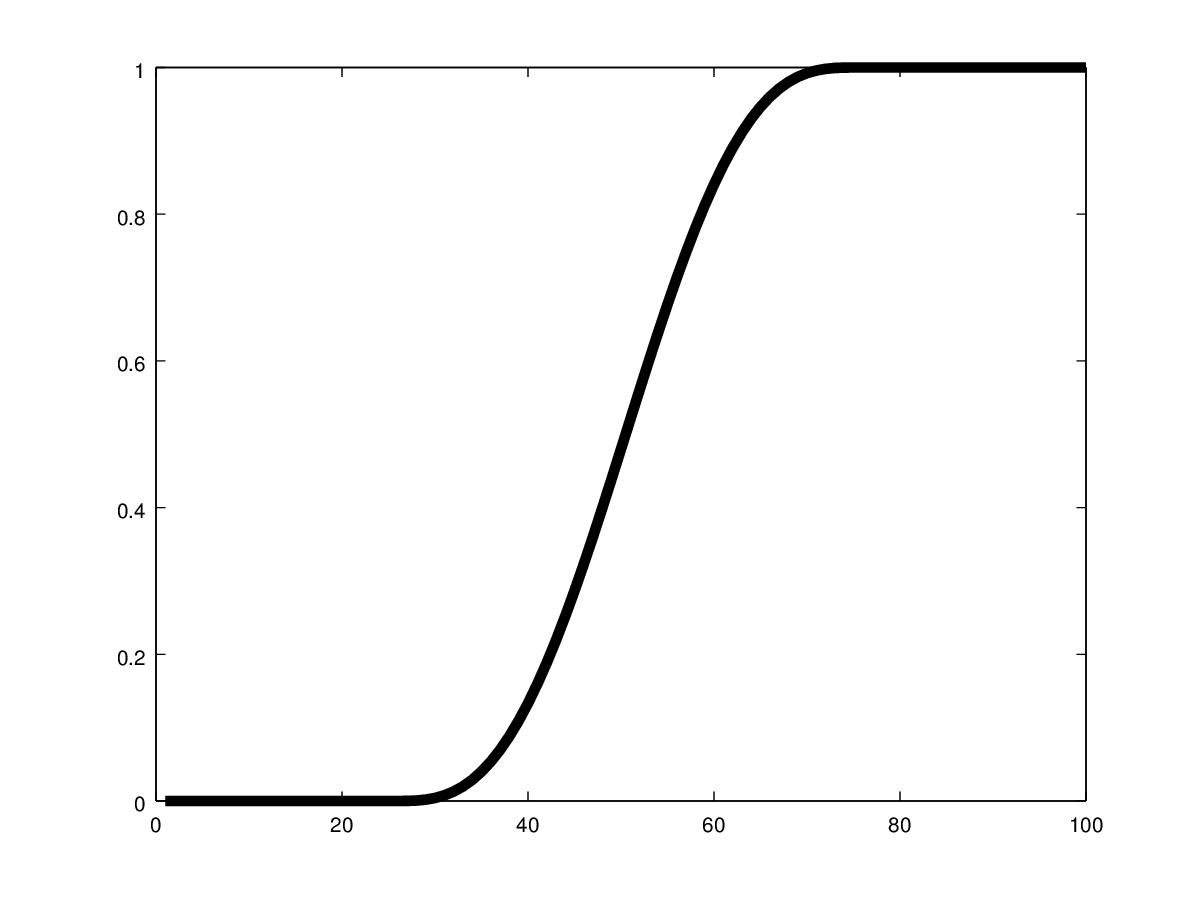
\includegraphics[width=0.3\textwidth]{graphics/heavside/heavside}
        \item Formula del punto medio Composita
          \[
          \mathcal{I}^n=\frac{1}{3V_0}\Delta x^3\sum_{j=1}^{|G_{\Delta x}|}F_j^n\delta_{\varepsilon}(u_j^n)
          \]
          
  \end{itemize}
Referenza: S. Osher e R. Fedkiw (2003).
\end{frame}


\begin{frame}{Flusso VPMCM nel caso della sfera}
  \begin{columns}[T]
    \begin{column}{6.5cm}
      \begin{exampleblock}{Caso semplificato, evoluzione della sfera}
        $S(R(t))$ famiglia di sfere in forma level-set
        \begin{itemize}
        \item $S_0=\{x\in\mathbb{R}^3| |x|^2-R_0^2=0\}$
        \item $V(R(t))=V_0\Rightarrow R(t)=R_0$
        \item $\mathcal{I}(\mathcal{H}(u),t)=2\frac{4\pi}{3V_0}R_0=2\left(\frac{4\pi}{3V_0}\right)^\frac{2}{3}$.
        \end{itemize}
      \end{exampleblock}
    \end{column}
    \begin{column}[T]{3.5cm}
      \begin{center}
        \only<2->{\animategraphics[autoplay,loop,width=1.0\textwidth,height=0.45\textheight]{0.8}{smooth/vpmcm/sphere/sphere}{0}{4}}
      \end{center}
  \end{column}
\end{columns}
\end{frame}

\begin{frame}{Consistenza generalizzata}
  \begin{definizione}[Consistenza]
    Sia $\phi\in C^{\infty}(\mathbb{R}^3\times[0,T])$ e $(\Delta
    x_m,\Delta t_m)\to (x,t)$ e  $(x_{n_m},t^{n_m})\to 0$  per
    $m\to\infty$, con $(\Delta x_m,\Delta t_m)$  sequenza di
    parametri di discretizzazione e $(x_{j_m},t^{n_m})$ sequenza di
    nodi. Allora lo schema $S$ è consistente con
    \[
    \phi_t(x,t)+F(x,D\phi,D^2\phi)=0
    \]
    se
    \[
    \left\{
    \begin{aligned}
      &\liminf_{m\to\infty}\frac{\phi(x_j,t_{n_m+1})-S_{j_m}(\phi^{n_m})}{\Delta
        t_m}\geq\phi_t(x,t)+F_*(x,D\phi,D^2\phi)
        \\
       &\limsup_{m\to\infty}\frac{\phi(x_j,t_{n_m+1})-S_{j_m}(\phi^{n_m})}{\Delta
          t_m}\leq\phi_t(x,t)+F^*(x,D\phi,D^2\phi)
    \end{aligned}
    \right.
    \]
    con $F_*$ inviluppo semicontinuo inferiore e $F^*$ inviluppo
    semicontinuo superiore.
  \end{definizione}
\end{frame}

\begin{frame}{Consistenza caso sfera con $Du\neq 0$ e
    $(Du)_1^2+(Du)_3^2\neq 0$}
  \begin{alertblock}{Schema sopra la soglia per la sfera}
   \[
     u_j^{n+1}=\frac{1}{4}\sum_{+,-}(I[u^n](x_j(1-C\Delta
     t)+\sqrt{2\Delta t}(\pm v_{j,1}^n\pm v_{j,2}^n))
    \]
    con $C=2\left(\frac{4\pi}{3V_0}\right)^\frac{2}{3}$.
  \end{alertblock}
  Supponiamo
  \begin{itemize}
    \item $u$ sufficientemente regolare con $|u_{tt}|<M$
    \item $||I[u^n](\cdot)-u(\cdot,t^n)||=O(\Delta x^2)$ errore di
      interpolazione 
    \item $|D_j^n-Du(x_j,t^n)|=O(\Delta x^2)$ errore approssimazione
      del gradiente
   \end{itemize}
  Osserviamo \\ 
      $|J_{\sigma}(p)|=\frac{1}{p_1^2+p_3^2}$ con $p=Du$ e
      $\sigma=[v_1,v_2]$ matrice $3\times 2$,  poichè vale
      $(D_j^n)_1^2+(D_j^n)_3^2\geq C\Delta x$ allora $\sigma$ è
      lipschitziana con $L_{\sigma_j^n}=\frac{1}{C\Delta x}$.  
 \end{frame}

\begin{frame}{Consistenza caso sopra la soglia}
Iniziamo la stima per \alert{$v_1+v_2=\sigma(D_j^n)b$} con $b=[1,1]^t$
\[
\begin{aligned}
  &I[u^n](x_j-x_jC\Delta t +\sqrt{2\Delta t}\sigma(D_j^n)b,t^n)=\\
  &u(x_j-x_jC\Delta t +\sqrt{2\Delta t}\sigma(Du(x_j,t^n))b,t^n)+\\
  &O(\Delta x^2) + O(\Delta x\Delta t^{\frac{1}{2}}) 
\end{aligned}
\]
Espansione di Taylor del terzo ordine otteniamo
\[
\begin{aligned}
&u(x_j-x_jC\Delta t +\sqrt{2\Delta
    t}(v_1+v_2),t^n)=u(x_j,t^n)+\\
&<Du(x_j,t^n),(v_1+v_2)>\sqrt{2\Delta t}+\Delta
  t<D^2u(x_j,t^n)(v_1+v_2),(v_1+v_2)>+\\
&-C<Du(x_j,t^n),x_j>\Delta t+T_3\Delta t^{\frac{3}{2}} +O(\Delta t^2)
\end{aligned}
\]
Ripetendo il calcolo per $(\pm v_1\pm v_2)$ e sommando abbiamo
\[
\begin{aligned}
S_j(u^n)&=u(x_j,t^n)+\Delta t(v_1^tD^2u(x_j,t^n)v_1+v_2^tD^2u(x_j,t^n)v_2-Cx^tDu(x_j,t^n))+\\
&O(\Delta x^2)+ O(\Delta x\Delta t^{\frac{1}{2}})+ O(\Delta t^2)
\end{aligned}
\]
\end{frame}

\begin{frame}{Consistenza caso sopra la soglia}
In conclusione utilizziamo la definizione di consistenza generalizzata
\[
\begin{aligned}
\frac{u(x_j,t^{n+1})-S_j(u^n)}{\Delta
  t}&=u_t(x_j,t^n)-v_1^tD^2u(x_j,t^n)v_1-v_2D^2u(x_j,t^n)v_2+\\
& Cx^tDu(x_j,t^n)+O(\Delta x^2\Delta t^{-1})+O(\Delta x\Delta
t^{-\frac{1}{2}})+O(\Delta t)
\end{aligned}
\]
\begin{alertblock}{Conclusione}
Poniamo ad esempio $\Delta t=\Delta x^{\alpha}$, affinchè il metodo
sia consistente per $(\Delta x,\Delta t)\to 0$ e $(x_j,t^n)\to (x,j)$
abbiamo 
\[
\begin{aligned}
&L_{\Delta x}\simeq\Delta x^{2-\alpha}+\Delta
x^{1-\frac{\alpha}{2}}+\Delta x \\
&\Delta x^{2-\alpha}\to 0\land\Delta x^{1-\frac{\alpha}{2}}\to 0\Rightarrow0<\alpha<2
\end{aligned}
\]
Quindi il metodo non richiede una CFL parabolica, per la quale
$\Delta t=O(\Delta x^2)$.
\end{alertblock}
\end{frame}


\section{Risultati Numerici}
\begin{frame}{Primi test sulla conservazione del volume}
  \begin{block}{Approssimazione del volume}
    Approssimiamo il volume, applicando la formula del punto medio
    composita a
    \[
    \int_{\Omega}(1-H(u(x)))dx\simeq\Delta x^3\sum_{i=1}^{|G_{\Delta x}|}(1-\tilde{H}(u(x)))
    \]
    con
    \[
    \tilde{H}(u)=
    \begin{cases}
      0 &u<-\varepsilon \\
      \frac{1}{2}+\frac{u}{2\varepsilon}+\frac{1}{2\pi}\sin{\frac{u\pi}{\varepsilon}}
        &-\varepsilon\leq u\leq\varepsilon \\
        1 &u>\varepsilon
    \end{cases}
    \]
 con $\varepsilon=1.5\Delta x$
  \end{block}
\end{frame}

\begin{frame}{Tabelle volume sfera}
\begin{table}[htb!]
\caption{Tabella per lo schema VPMCM. Evoluzione di una sfera.}
\label{tab:cp4-sc1-01}
\[
\begin{array}{*{6}{c}l}
    \toprule
    \text{time} &\text{nodi} &\Delta t &\text{iter}
    &\text{CPUs}&\text{VolE$_{\infty}$} &\text{VolE\ped{rel}} \\
     \midrule
     0.1        & 80         & 0.10    & 1          & 1,0s
     &1.1e^{-01} & 3.1e^{-03} \\ 
     0.2        &            &         & 2          & 3.7s
     &2.3e^{-01} & 6.9e^{-03} \\
     0.5        &            &         & 5          & 8,8s
     &7.5e^{-01} & 2.3e^{-02} \\ 
     1.0        &            &         & 10         & 21s
     &2.5e^{-00} & 7.6e^{-02} \\
    \midrule
     0.1        & 180        & 0.04    & 3          & 53s
     &1.1e^{-01} & 3.3e^{-03} \\ 
     0.2        &            &         & 5          & 91s
     &1.8e^{-01} & 5.3e^{-03} \\
     0.5        &            &         & 12         & 173s
     &2.9e^{-01} & 8.6e^{-03}  \\ 
     1.0        &            &         & 23         & 566s
     &2.3e^{-01} & 7.1e^{-03}  \\
    \bottomrule
\end{array}
\]
\end{table}
\end{frame}

\begin{frame}{\emph{Denoising} superfici geometriche}
  \begin{columns}[T]
    \begin{column}{4cm}
      \begin{block}{Rumore \emph{random}}
        Funzione che genera sfere di rumore random
        \begin{itemize}
        \item Numero di sfere
        \item Raggio delle sfere random in un range tra $[0$,raggioInput$]$ 
        \item Valore di rumore random tra $[0$,noiseInput$]$
        \end{itemize}
      \end{block}
    \end{column}
   \begin{column}{6cm}
     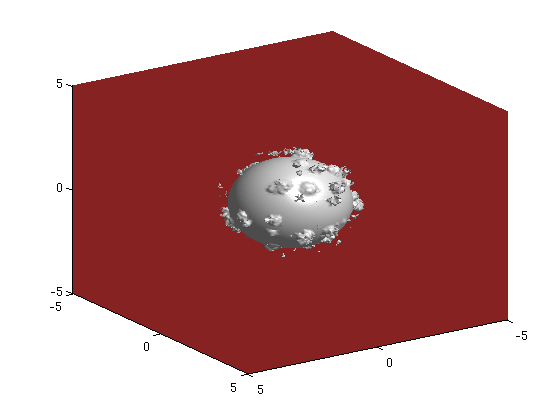
\includegraphics[width=1.0\textwidth]{noise/randNoise/mcm/sphere/sphere100r-0-00}
   \end{column}
  \end{columns}
\end{frame}

\begin{frame}{VPMCM vs MCM}
\begin{columns}[T]
  \begin{column}{5cm}
    \centering
    \only<1>{\animategraphics[autoplay,loop,width=1.0\textwidth,height=0.55\textheight]{0.8}{noise/randNoise/mcm/sphere/sphere100r-}{0}{5}}
    \end{column}
  \begin{column}[T]{5cm}
    \centering
    \only<1>{\animategraphics[autoplay,loop,width=1.0\textwidth,height=0.55\textheight]{0.8}{noise/randNoise/vpmcm/sphere/sphere100r-}{0}{5}}
    \end{column}
 \end{columns}
\begin{columns}[T]
  \begin{column}{5cm}
    \centering
    \only<2>{\animategraphics[autoplay,loop,width=1.0\textwidth,height=0.55\textheight]{0.8}{noise/randNoise/mcm/dumbbell/dumb100r-}{0}{4}}
    \end{column}
  \begin{column}[T]{5cm}
    \centering
    \only<2>{\animategraphics[autoplay,loop,width=1.0\textwidth,height=0.55\textheight]{0.8}{noise/randNoise/vpmcm/dumbbell/dumb100r-}{0}{4}}
    \end{column}
  \end{columns}
\end{frame}

\begin{frame}{\emph{Denoising} superfici geometriche}
 \begin{columns}[T]
   \begin{column}{4cm}
     \begin{block}{Rumore \emph{gaussiano}}
       Il rumore gaussiano è stato generato usando la funzione
       \emph{imnoise} di MATLAB, che simula il rumore con una distribuzione
       gaussiana.
     \end{block}
     \end{column}
   \begin{column}[T]{6cm}
     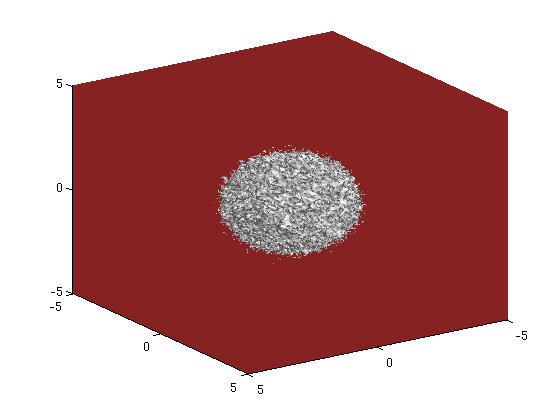
\includegraphics[width=1.0\textwidth]{noise/imnoise/mcm/sphere/sphere100i-0-00}
   \end{column}
 \end{columns}
\end{frame}

\begin{frame}{VPMCM vs MCM}
 \begin{columns}[T]
  \begin{column}{5cm}
    \centering
    \only<1>{\animategraphics[autoplay,loop,width=1.0\textwidth,height=0.55\textheight]{0.8}{noise/imnoise/mcm/sphere/sphere100i-}{0}{5}}
    \end{column}
  \begin{column}[T]{5cm}
    \centering
    \only<1>{\animategraphics[autoplay,loop,width=1.0\textwidth,height=0.55\textheight]{0.8}{noise/imnoise/vpmcm/sphere/sphere100i-}{0}{5}}
    \end{column}
 \end{columns}
\begin{columns}[T]
  \begin{column}{5cm}
    \centering
    \only<2>{\animategraphics[autoplay,loop,width=1.0\textwidth,height=0.55\textheight]{0.8}{noise/imnoise/mcm/dumbbell/dumb149i-}{0}{5}}
    \end{column}
  \begin{column}[T]{5cm}
    \centering
    \only<2>{\animategraphics[autoplay,loop,width=1.0\textwidth,height=0.55\textheight]{0.8}{noise/imnoise/vpmcm/dumbbell/dumb149i-}{0}{5}}
    \end{column}
  \end{columns}
\end{frame}

\begin{frame}{Immagine reale 3D}
 \begin{columns}[T]
    \begin{column}{4cm}
      \begin{block}{\emph{Gargolye}}
        \begin{itemize}
        \item Immagine ottenuta da uno scanner 3D
        \item La funzione levle-set non è regolare come le precedenti 
        \item Il metodo si comporta bene solo per poco iterazioni
        \item Abbiamo usato rumori piccoli
        \item Non sono molto evidenti le differenze con MCM
        \end{itemize}
      \end{block}
    \end{column}
   \begin{column}{6cm}
     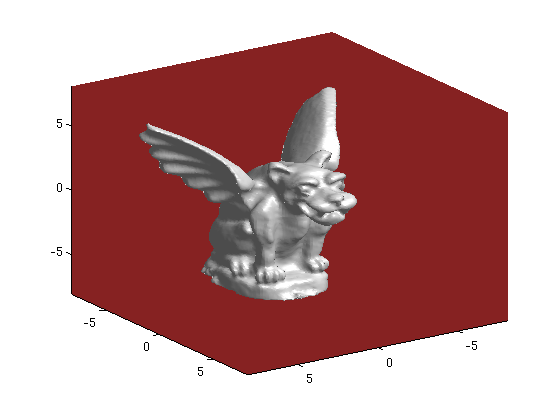
\includegraphics[width=1.0\textwidth]{smooth/mcm/gargolye/garg149-0-00}
   \end{column}
  \end{columns}
\end{frame}

\begin{frame}{Immagine reale 3D}
  \begin{columns}[T]
  \begin{column}{5cm}
    \centering
    \only<1->{\animategraphics[autoplay,loop,width=1.0\textwidth,height=0.55\textheight]{0.8}{noise/imnoise/vpmcm/gargolye/garg149i-}{0}{4}}
    \end{column}
  \begin{column}[T]{5cm}
    \centering
    \only<2>{\animategraphics[autoplay,loop,width=1.0\textwidth,height=0.55\textheight]{0.8}{noise/randNoise/vpmcm/gargolye/garg149r3-}{0}{3}}
    \end{column}
 \end{columns}
\end{frame}

%
%
% Reference 
\begin{frame}{Referenze}
\begin{thebibliography}{bella}
\bibitem{Crandallions}[Crandall, 1992]
  Michle C. Crandall, Ishii Hitoshi e Lions P.L.
  \newblock \emph{User's guide to viscosity solutions of second order
    partial differantial equations}, 1992.

\bibitem{Goldbach1742}[Oscher, 2003] 
  Osher Stanley e Fedkiw Ronald
  \newblock \emph{Level set Methods and Dynamic Implicit Surface}, 2003.

\bibitem{Goldbach1742}[Sapiro, 2001] 
  Sapiro Guillermo
  \newblock \emph{Geometric Partial Differantial Equation and Image
    Analysis}, 2003.

\bibitem{Goldbach1742}[Carlini, 2010] 
  E. Carlini, M. Falcone e R. Ferretti
  \newblock \emph{Convergence of large time-step scheme for mean
    curvature motion}, 2010.

\end{thebibliography}
\end{frame}
%
%
%
\end{document}


